% Created by tikzDevice version 0.12.3.1 on 2023-03-16 10:38:59
% !TEX encoding = UTF-8 Unicode
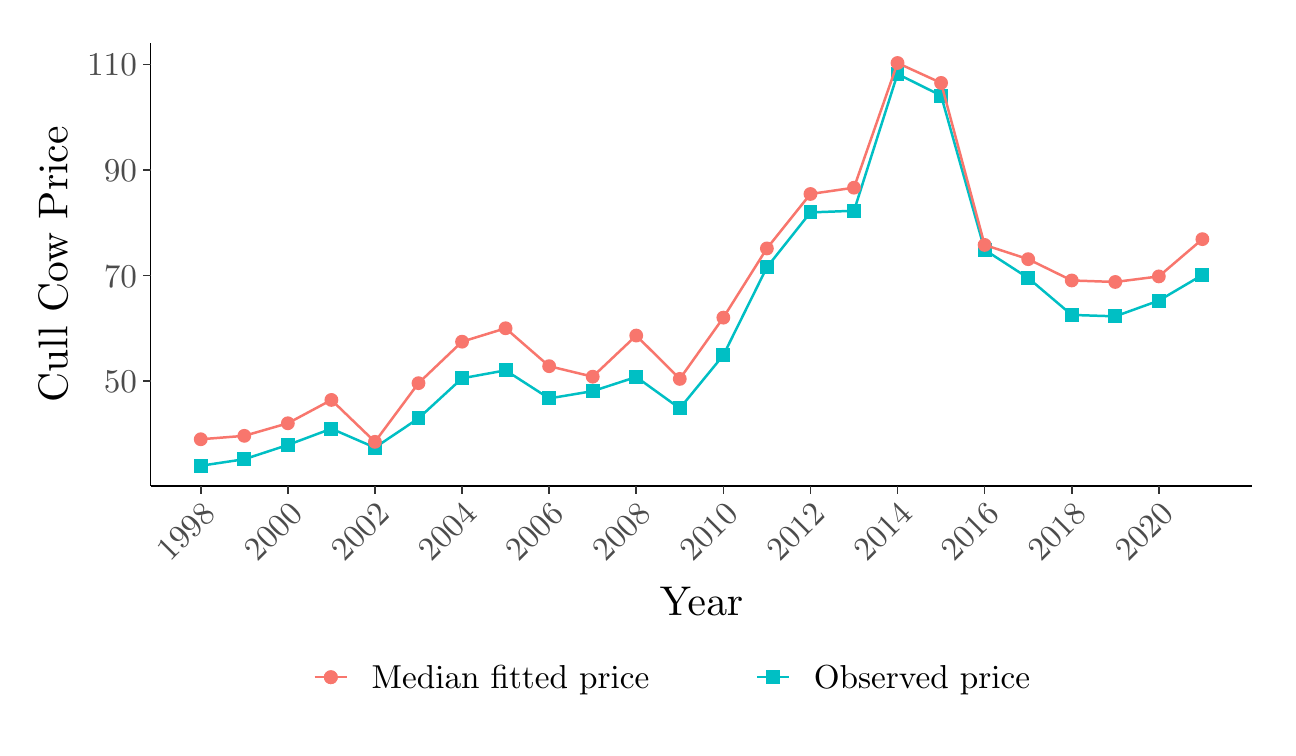
\begin{tikzpicture}[x=1pt,y=1pt]
\definecolor{fillColor}{RGB}{255,255,255}
\path[use as bounding box,fill=fillColor,fill opacity=0.00] (0,0) rectangle (448.07,252.94);
\begin{scope}
\path[clip] (  0.00,  0.00) rectangle (448.07,252.94);
\definecolor{drawColor}{RGB}{255,255,255}
\definecolor{fillColor}{RGB}{255,255,255}

\path[draw=drawColor,line width= 0.6pt,line join=round,line cap=round,fill=fillColor] (  0.00,  0.00) rectangle (448.07,252.94);
\end{scope}
\begin{scope}
\path[clip] ( 44.44, 87.36) rectangle (442.57,247.45);
\definecolor{fillColor}{RGB}{255,255,255}

\path[fill=fillColor] ( 44.44, 87.36) rectangle (442.57,247.44);
\definecolor{drawColor}{RGB}{0,191,196}

\path[draw=drawColor,line width= 0.9pt,line join=round] ( 62.54, 94.64) --
	( 78.28, 97.00) --
	( 94.01,102.15) --
	(109.75,108.03) --
	(125.48,101.20) --
	(141.22,111.76) --
	(156.96,126.24) --
	(172.69,129.12) --
	(188.43,118.97) --
	(204.17,121.60) --
	(219.90,126.72) --
	(235.64,115.37) --
	(251.38,134.59) --
	(267.11,166.35) --
	(282.85,186.18) --
	(298.59,186.77) --
	(314.32,236.22) --
	(330.06,228.38) --
	(345.79,172.66) --
	(361.53,162.49) --
	(377.27,149.14) --
	(393.00,148.63) --
	(408.74,154.31) --
	(424.48,163.58);
\definecolor{fillColor}{RGB}{0,191,196}

\path[fill=fillColor] ( 60.04, 92.14) --
	( 65.04, 92.14) --
	( 65.04, 97.13) --
	( 60.04, 97.13) --
	cycle;

\path[fill=fillColor] ( 75.78, 94.50) --
	( 80.77, 94.50) --
	( 80.77, 99.50) --
	( 75.78, 99.50) --
	cycle;

\path[fill=fillColor] ( 91.51, 99.65) --
	( 96.51, 99.65) --
	( 96.51,104.65) --
	( 91.51,104.65) --
	cycle;

\path[fill=fillColor] (107.25,105.53) --
	(112.25,105.53) --
	(112.25,110.52) --
	(107.25,110.52) --
	cycle;

\path[fill=fillColor] (122.99, 98.70) --
	(127.98, 98.70) --
	(127.98,103.70) --
	(122.99,103.70) --
	cycle;

\path[fill=fillColor] (138.72,109.27) --
	(143.72,109.27) --
	(143.72,114.26) --
	(138.72,114.26) --
	cycle;

\path[fill=fillColor] (154.46,123.74) --
	(159.46,123.74) --
	(159.46,128.74) --
	(154.46,128.74) --
	cycle;

\path[fill=fillColor] (170.20,126.62) --
	(175.19,126.62) --
	(175.19,131.62) --
	(170.20,131.62) --
	cycle;

\path[fill=fillColor] (185.93,116.47) --
	(190.93,116.47) --
	(190.93,121.47) --
	(185.93,121.47) --
	cycle;

\path[fill=fillColor] (201.67,119.11) --
	(206.66,119.11) --
	(206.66,124.10) --
	(201.67,124.10) --
	cycle;

\path[fill=fillColor] (217.41,124.22) --
	(222.40,124.22) --
	(222.40,129.21) --
	(217.41,129.21) --
	cycle;

\path[fill=fillColor] (233.14,112.87) --
	(238.14,112.87) --
	(238.14,117.87) --
	(233.14,117.87) --
	cycle;

\path[fill=fillColor] (248.88,132.09) --
	(253.87,132.09) --
	(253.87,137.09) --
	(248.88,137.09) --
	cycle;

\path[fill=fillColor] (264.62,163.85) --
	(269.61,163.85) --
	(269.61,168.84) --
	(264.62,168.84) --
	cycle;

\path[fill=fillColor] (280.35,183.68) --
	(285.35,183.68) --
	(285.35,188.68) --
	(280.35,188.68) --
	cycle;

\path[fill=fillColor] (296.09,184.27) --
	(301.08,184.27) --
	(301.08,189.27) --
	(296.09,189.27) --
	cycle;

\path[fill=fillColor] (311.82,233.72) --
	(316.82,233.72) --
	(316.82,238.72) --
	(311.82,238.72) --
	cycle;

\path[fill=fillColor] (327.56,225.89) --
	(332.56,225.89) --
	(332.56,230.88) --
	(327.56,230.88) --
	cycle;

\path[fill=fillColor] (343.30,170.16) --
	(348.29,170.16) --
	(348.29,175.16) --
	(343.30,175.16) --
	cycle;

\path[fill=fillColor] (359.03,160.00) --
	(364.03,160.00) --
	(364.03,164.99) --
	(359.03,164.99) --
	cycle;

\path[fill=fillColor] (374.77,146.65) --
	(379.77,146.65) --
	(379.77,151.64) --
	(374.77,151.64) --
	cycle;

\path[fill=fillColor] (390.51,146.13) --
	(395.50,146.13) --
	(395.50,151.13) --
	(390.51,151.13) --
	cycle;

\path[fill=fillColor] (406.24,151.81) --
	(411.24,151.81) --
	(411.24,156.81) --
	(406.24,156.81) --
	cycle;

\path[fill=fillColor] (421.98,161.08) --
	(426.97,161.08) --
	(426.97,166.08) --
	(421.98,166.08) --
	cycle;
\definecolor{drawColor}{RGB}{248,118,109}

\path[draw=drawColor,line width= 0.9pt,line join=round] ( 62.54,104.21) --
	( 78.28,105.45) --
	( 94.01,109.99) --
	(109.75,118.42) --
	(125.48,103.28) --
	(141.22,124.48) --
	(156.96,139.47) --
	(172.69,144.32) --
	(188.43,130.62) --
	(204.17,126.82) --
	(219.90,141.69) --
	(235.64,126.02) --
	(251.38,148.16) --
	(267.11,173.17) --
	(282.85,192.84) --
	(298.59,195.12) --
	(314.32,240.17) --
	(330.06,232.97) --
	(345.79,174.43) --
	(361.53,169.29) --
	(377.27,161.59) --
	(393.00,161.05) --
	(408.74,163.06) --
	(424.48,176.52);
\definecolor{fillColor}{RGB}{248,118,109}

\path[fill=fillColor] ( 62.54,104.21) circle (  2.50);

\path[fill=fillColor] ( 78.28,105.45) circle (  2.50);

\path[fill=fillColor] ( 94.01,109.99) circle (  2.50);

\path[fill=fillColor] (109.75,118.42) circle (  2.50);

\path[fill=fillColor] (125.48,103.28) circle (  2.50);

\path[fill=fillColor] (141.22,124.48) circle (  2.50);

\path[fill=fillColor] (156.96,139.47) circle (  2.50);

\path[fill=fillColor] (172.69,144.32) circle (  2.50);

\path[fill=fillColor] (188.43,130.62) circle (  2.50);

\path[fill=fillColor] (204.17,126.82) circle (  2.50);

\path[fill=fillColor] (219.90,141.69) circle (  2.50);

\path[fill=fillColor] (235.64,126.02) circle (  2.50);

\path[fill=fillColor] (251.38,148.16) circle (  2.50);

\path[fill=fillColor] (267.11,173.17) circle (  2.50);

\path[fill=fillColor] (282.85,192.84) circle (  2.50);

\path[fill=fillColor] (298.59,195.12) circle (  2.50);

\path[fill=fillColor] (314.32,240.17) circle (  2.50);

\path[fill=fillColor] (330.06,232.97) circle (  2.50);

\path[fill=fillColor] (345.79,174.43) circle (  2.50);

\path[fill=fillColor] (361.53,169.29) circle (  2.50);

\path[fill=fillColor] (377.27,161.59) circle (  2.50);

\path[fill=fillColor] (393.00,161.05) circle (  2.50);

\path[fill=fillColor] (408.74,163.06) circle (  2.50);

\path[fill=fillColor] (424.48,176.52) circle (  2.50);
\end{scope}
\begin{scope}
\path[clip] (  0.00,  0.00) rectangle (448.07,252.94);
\definecolor{drawColor}{RGB}{0,0,0}

\path[draw=drawColor,line width= 0.6pt,line join=round] ( 44.44, 87.36) --
	( 44.44,247.45);
\end{scope}
\begin{scope}
\path[clip] (  0.00,  0.00) rectangle (448.07,252.94);
\definecolor{drawColor}{gray}{0.30}

\node[text=drawColor,anchor=base east,inner sep=0pt, outer sep=0pt, scale=  1.20] at ( 39.49,121.06) {50};

\node[text=drawColor,anchor=base east,inner sep=0pt, outer sep=0pt, scale=  1.20] at ( 39.49,159.20) {70};

\node[text=drawColor,anchor=base east,inner sep=0pt, outer sep=0pt, scale=  1.20] at ( 39.49,197.34) {90};

\node[text=drawColor,anchor=base east,inner sep=0pt, outer sep=0pt, scale=  1.20] at ( 39.49,235.48) {110};
\end{scope}
\begin{scope}
\path[clip] (  0.00,  0.00) rectangle (448.07,252.94);
\definecolor{drawColor}{gray}{0.20}

\path[draw=drawColor,line width= 0.6pt,line join=round] ( 41.69,125.19) --
	( 44.44,125.19);

\path[draw=drawColor,line width= 0.6pt,line join=round] ( 41.69,163.33) --
	( 44.44,163.33);

\path[draw=drawColor,line width= 0.6pt,line join=round] ( 41.69,201.47) --
	( 44.44,201.47);

\path[draw=drawColor,line width= 0.6pt,line join=round] ( 41.69,239.62) --
	( 44.44,239.62);
\end{scope}
\begin{scope}
\path[clip] (  0.00,  0.00) rectangle (448.07,252.94);
\definecolor{drawColor}{RGB}{0,0,0}

\path[draw=drawColor,line width= 0.6pt,line join=round] ( 44.44, 87.36) --
	(442.57, 87.36);
\end{scope}
\begin{scope}
\path[clip] (  0.00,  0.00) rectangle (448.07,252.94);
\definecolor{drawColor}{gray}{0.20}

\path[draw=drawColor,line width= 0.6pt,line join=round] ( 62.54, 84.61) --
	( 62.54, 87.36);

\path[draw=drawColor,line width= 0.6pt,line join=round] ( 94.01, 84.61) --
	( 94.01, 87.36);

\path[draw=drawColor,line width= 0.6pt,line join=round] (125.48, 84.61) --
	(125.48, 87.36);

\path[draw=drawColor,line width= 0.6pt,line join=round] (156.96, 84.61) --
	(156.96, 87.36);

\path[draw=drawColor,line width= 0.6pt,line join=round] (188.43, 84.61) --
	(188.43, 87.36);

\path[draw=drawColor,line width= 0.6pt,line join=round] (219.90, 84.61) --
	(219.90, 87.36);

\path[draw=drawColor,line width= 0.6pt,line join=round] (251.38, 84.61) --
	(251.38, 87.36);

\path[draw=drawColor,line width= 0.6pt,line join=round] (282.85, 84.61) --
	(282.85, 87.36);

\path[draw=drawColor,line width= 0.6pt,line join=round] (314.32, 84.61) --
	(314.32, 87.36);

\path[draw=drawColor,line width= 0.6pt,line join=round] (345.79, 84.61) --
	(345.79, 87.36);

\path[draw=drawColor,line width= 0.6pt,line join=round] (377.27, 84.61) --
	(377.27, 87.36);

\path[draw=drawColor,line width= 0.6pt,line join=round] (408.74, 84.61) --
	(408.74, 87.36);
\end{scope}
\begin{scope}
\path[clip] (  0.00,  0.00) rectangle (448.07,252.94);
\definecolor{drawColor}{gray}{0.30}

\node[text=drawColor,rotate= 45.00,anchor=base east,inner sep=0pt, outer sep=0pt, scale=  1.20] at ( 68.38, 76.57) {1998};

\node[text=drawColor,rotate= 45.00,anchor=base east,inner sep=0pt, outer sep=0pt, scale=  1.20] at ( 99.86, 76.57) {2000};

\node[text=drawColor,rotate= 45.00,anchor=base east,inner sep=0pt, outer sep=0pt, scale=  1.20] at (131.33, 76.57) {2002};

\node[text=drawColor,rotate= 45.00,anchor=base east,inner sep=0pt, outer sep=0pt, scale=  1.20] at (162.80, 76.57) {2004};

\node[text=drawColor,rotate= 45.00,anchor=base east,inner sep=0pt, outer sep=0pt, scale=  1.20] at (194.27, 76.57) {2006};

\node[text=drawColor,rotate= 45.00,anchor=base east,inner sep=0pt, outer sep=0pt, scale=  1.20] at (225.75, 76.57) {2008};

\node[text=drawColor,rotate= 45.00,anchor=base east,inner sep=0pt, outer sep=0pt, scale=  1.20] at (257.22, 76.57) {2010};

\node[text=drawColor,rotate= 45.00,anchor=base east,inner sep=0pt, outer sep=0pt, scale=  1.20] at (288.69, 76.57) {2012};

\node[text=drawColor,rotate= 45.00,anchor=base east,inner sep=0pt, outer sep=0pt, scale=  1.20] at (320.17, 76.57) {2014};

\node[text=drawColor,rotate= 45.00,anchor=base east,inner sep=0pt, outer sep=0pt, scale=  1.20] at (351.64, 76.57) {2016};

\node[text=drawColor,rotate= 45.00,anchor=base east,inner sep=0pt, outer sep=0pt, scale=  1.20] at (383.11, 76.57) {2018};

\node[text=drawColor,rotate= 45.00,anchor=base east,inner sep=0pt, outer sep=0pt, scale=  1.20] at (414.58, 76.57) {2020};
\end{scope}
\begin{scope}
\path[clip] (  0.00,  0.00) rectangle (448.07,252.94);
\definecolor{drawColor}{RGB}{0,0,0}

\node[text=drawColor,anchor=base,inner sep=0pt, outer sep=0pt, scale=  1.50] at (243.51, 40.50) {Year};
\end{scope}
\begin{scope}
\path[clip] (  0.00,  0.00) rectangle (448.07,252.94);
\definecolor{drawColor}{RGB}{0,0,0}

\node[text=drawColor,rotate= 90.00,anchor=base,inner sep=0pt, outer sep=0pt, scale=  1.50] at ( 14.37,167.40) {Cull Cow Price};
\end{scope}
\begin{scope}
\path[clip] (  0.00,  0.00) rectangle (448.07,252.94);
\definecolor{fillColor}{RGB}{255,255,255}

\path[fill=fillColor] ( 89.33,  5.50) rectangle (397.69, 30.95);
\end{scope}
\begin{scope}
\path[clip] (  0.00,  0.00) rectangle (448.07,252.94);
\definecolor{drawColor}{RGB}{248,118,109}

\path[draw=drawColor,line width= 0.9pt,line join=round] (103.77, 18.23) -- (115.33, 18.23);
\end{scope}
\begin{scope}
\path[clip] (  0.00,  0.00) rectangle (448.07,252.94);
\definecolor{fillColor}{RGB}{248,118,109}

\path[fill=fillColor] (109.55, 18.23) circle (  2.50);
\end{scope}
\begin{scope}
\path[clip] (  0.00,  0.00) rectangle (448.07,252.94);
\definecolor{drawColor}{RGB}{248,118,109}

\path[draw=drawColor,line width= 0.9pt,line join=round] (103.77, 18.23) -- (115.33, 18.23);
\end{scope}
\begin{scope}
\path[clip] (  0.00,  0.00) rectangle (448.07,252.94);
\definecolor{fillColor}{RGB}{248,118,109}

\path[fill=fillColor] (109.55, 18.23) circle (  2.50);
\end{scope}
\begin{scope}
\path[clip] (  0.00,  0.00) rectangle (448.07,252.94);
\definecolor{drawColor}{RGB}{0,191,196}

\path[draw=drawColor,line width= 0.9pt,line join=round] (263.57, 18.23) -- (275.13, 18.23);
\end{scope}
\begin{scope}
\path[clip] (  0.00,  0.00) rectangle (448.07,252.94);
\definecolor{fillColor}{RGB}{0,191,196}

\path[fill=fillColor] (266.85, 15.73) --
	(271.85, 15.73) --
	(271.85, 20.72) --
	(266.85, 20.72) --
	cycle;
\end{scope}
\begin{scope}
\path[clip] (  0.00,  0.00) rectangle (448.07,252.94);
\definecolor{drawColor}{RGB}{0,191,196}

\path[draw=drawColor,line width= 0.9pt,line join=round] (263.57, 18.23) -- (275.13, 18.23);
\end{scope}
\begin{scope}
\path[clip] (  0.00,  0.00) rectangle (448.07,252.94);
\definecolor{fillColor}{RGB}{0,191,196}

\path[fill=fillColor] (266.85, 15.73) --
	(271.85, 15.73) --
	(271.85, 20.72) --
	(266.85, 20.72) --
	cycle;
\end{scope}
\begin{scope}
\path[clip] (  0.00,  0.00) rectangle (448.07,252.94);
\definecolor{drawColor}{RGB}{0,0,0}

\node[text=drawColor,anchor=base west,inner sep=0pt, outer sep=0pt, scale=  1.20] at (124.28, 14.09) {Median fitted price};
\end{scope}
\begin{scope}
\path[clip] (  0.00,  0.00) rectangle (448.07,252.94);
\definecolor{drawColor}{RGB}{0,0,0}

\node[text=drawColor,anchor=base west,inner sep=0pt, outer sep=0pt, scale=  1.20] at (284.08, 14.09) {Observed price};
\end{scope}
\end{tikzpicture}
